\documentclass[12pt]{article}
\usepackage[margin=1in]{geometry}
\usepackage{amsmath,amssymb,amsthm}
\usepackage{graphicx}
\usepackage{tikz}
\usetikzlibrary{arrows.meta,shapes,positioning,calc}
\usepackage{booktabs}
\usepackage{natbib}
\usepackage{hyperref}
\usepackage{xcolor}
\usepackage{enumerate}

\newtheorem{theorem}{Theorem}
\newtheorem{proposition}{Proposition}
\newtheorem{definition}{Definition}

\title{\textbf{Emergent Codes:\\How Digital Information Arises from High-Dimensional Prebiotic Chemistry}}

\author{Ian Todd\\
Sydney Medical School\\
University of Sydney\\
Sydney, NSW, Australia\\
\texttt{itod2305@uni.sydney.edu.au}}

\date{}

\begin{document}

\maketitle

\begin{abstract}
The origin of genetic codes is often framed as a problem of engineering: how did chemistry come to \textit{encode} information? We argue this framing inverts the actual causality. Digital codes are not built into chemistry; they emerge from the projection of high-dimensional dynamics onto low-dimensional boundaries. When diverse chemical species track a common external forcing (solar and tidal cycles), their collective response forms a high-dimensional attractor---many distinct ``ways to track the sun.'' At boundaries (membranes, mineral surfaces), this high-dimensional dynamics projects onto discrete symbols through bistable physical mechanisms. The transition to life occurs when compartmentalization allows chemistry to swap the external attractor for an endogenously generated one. We develop this framework mathematically, showing that emergent digitality is a generic consequence of dimensionality reduction at interfaces, and discuss implications for understanding the origin of biological information.
\end{abstract}

\textbf{Keywords:} Origin of life; genetic code; emergence; dimensionality; prebiotic chemistry; information

%==============================================================================
\section{Introduction}
%==============================================================================

The genetic code presents a puzzle: how did discrete, symbolic information arise from continuous chemical processes? Standard approaches seek specific reaction mechanisms---particular molecules that could serve as primordial ``bits'' \citep{eigen1971selforganization, kauffman1993origins}. This framing assumes that digitality must be engineered into chemistry. Recent work has emphasized the algorithmic and informational aspects of life's origin \citep{walker2013algorithmic, schrodinger1944life}, yet the mechanism by which continuous chemistry produces discrete codes remains unclear.

We argue for an alternative view: digital codes are not fundamental but \textit{emergent}. They arise inevitably when high-dimensional continuous dynamics project onto low-dimensional observables at boundaries. The discreteness is not a property of the chemistry but of the interface between complex internal dynamics and simple readouts.

This perspective reframes the origin-of-codes problem. Rather than asking ``what chemistry produces digital information?'' we ask ``why do boundaries inevitably discretize high-dimensional dynamics?'' The answer involves well-understood mathematics: projection from high to low dimensions, through bistable mechanisms, is a discretizing operation.

The structure of the paper is as follows. Section 2 develops the concept of high-dimensional attractors from common forcing. Section 3 shows how digital symbols emerge at boundaries. Section 4 describes the transition from externally-organized to self-organized systems. Section 5 discusses experimental implications. Section 6 concludes with broader implications for understanding biological information.

%==============================================================================
\section{High-Dimensional Attractors from Common Forcing}
%==============================================================================

\subsection{The Prebiotic Setup}

Consider the chemical environment of early Earth \citep{ruizmirazo2014prebiotic, pross2012toward}:
\begin{itemize}
    \item \textbf{Diverse chemistry}: Amino acids, sugars, nucleobases, lipids, metal ions, thiols, phosphates---hundreds of species from atmospheric synthesis, meteoric delivery, and hydrothermal processes \citep{miller1953production, chyba1992endogenous}
    \item \textbf{Common forcing}: Solar radiation (day/night UV flux, temperature cycling), tidal cycles (wet/dry, concentration/dilution), seasonal variation
    \item \textbf{Cross-reactivity}: Extensive reaction networks---condensation, complexation, redox chemistry, catalysis
\end{itemize}

Each chemical species responds to the external forcing differently:
\begin{itemize}
    \item Amino acids undergo photodegradation during daylight, condensation during dry phases
    \item Sugar isomerization rates depend on temperature; formose branching is UV-sensitive
    \item Nucleobase chemistry is driven by UV absorption; metal complexation shifts with redox state
    \item Lipid phase transitions track temperature; self-assembly depends on concentration
\end{itemize}

\subsection{Formation of High-Dimensional Attractors}

When multiple species with distinct response characteristics are coupled through cross-reactions, and all track a common external rhythm, the collective dynamics forms a high-dimensional attractor.

Let $\mathbf{x}(t) \in \mathbb{R}^n$ represent the concentrations of $n$ chemical species. Under periodic forcing $F(t) = F(t+T)$, the dynamics satisfy:
\begin{equation}
    \frac{d\mathbf{x}}{dt} = \mathbf{f}(\mathbf{x}) + \mathbf{g}(\mathbf{x})F(t)
\end{equation}
where $\mathbf{f}$ captures internal reaction dynamics and $\mathbf{g}$ the forcing response.

For sufficiently diverse chemistry (large $n$, varied $\mathbf{g}$), the system admits multiple stable entrainment modes---different ways to synchronize with the external forcing. These modes form an attractor manifold $\mathcal{A} \subset \mathbb{R}^n$ with effective dimension $d_{\text{eff}} \ll n$ but still $d_{\text{eff}} \gg 1$.

\begin{figure}[h]
\centering
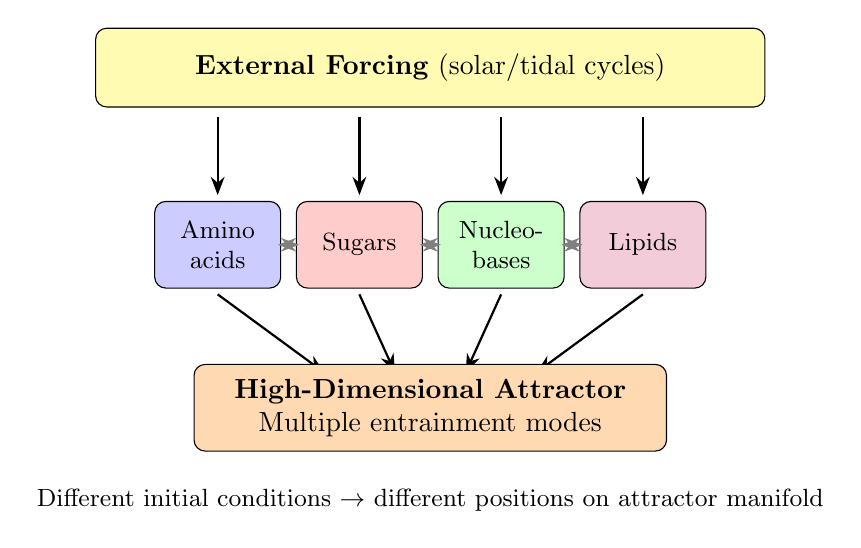
\begin{tikzpicture}[scale=0.9]
    % Sun forcing at top
    \node[draw, rounded corners, fill=yellow!30, minimum width=8.5cm, minimum height=1cm] at (0,4.2) {\textbf{External Forcing} (solar/tidal cycles)};

    % Arrows down to different chemistries
    \draw[-{Stealth}, thick] (-3,3.5) -- (-3,2.4);
    \draw[-{Stealth}, thick] (-1,3.5) -- (-1,2.4);
    \draw[-{Stealth}, thick] (1,3.5) -- (1,2.4);
    \draw[-{Stealth}, thick] (3,3.5) -- (3,2.4);

    % Different chemistry boxes - spread further apart
    \node[draw, rounded corners, fill=blue!20, minimum width=1.6cm, minimum height=1.1cm, align=center, font=\small] at (-3,1.7) {Amino\\acids};
    \node[draw, rounded corners, fill=red!20, minimum width=1.6cm, minimum height=1.1cm, align=center, font=\small] at (-1,1.7) {Sugars};
    \node[draw, rounded corners, fill=green!20, minimum width=1.6cm, minimum height=1.1cm, align=center, font=\small] at (1,1.7) {Nucleo-\\bases};
    \node[draw, rounded corners, fill=purple!20, minimum width=1.6cm, minimum height=1.1cm, align=center, font=\small] at (3,1.7) {Lipids};

    % Cross-coupling arrows - now visible between the boxes
    \draw[{Stealth}-{Stealth}, gray, thick] (-2.15,1.7) -- (-1.85,1.7);
    \draw[{Stealth}-{Stealth}, gray, thick] (-0.15,1.7) -- (0.15,1.7);
    \draw[{Stealth}-{Stealth}, gray, thick] (1.85,1.7) -- (2.15,1.7);

    % Arrows down to attractor
    \draw[-{Stealth}, thick] (-3,1.0) -- (-1.5,-0.1);
    \draw[-{Stealth}, thick] (-1,1.0) -- (-0.5,-0.1);
    \draw[-{Stealth}, thick] (1,1.0) -- (0.5,-0.1);
    \draw[-{Stealth}, thick] (3,1.0) -- (1.5,-0.1);

    % High-D attractor
    \node[draw, rounded corners, fill=orange!30, minimum width=6cm, minimum height=1.1cm, align=center] at (0,-0.6) {\textbf{High-Dimensional Attractor}\\Multiple entrainment modes};

    % Label
    \node[font=\small, align=center] at (0,-1.9) {Different initial conditions $\to$ different positions on attractor manifold};
\end{tikzpicture}
\caption{Diverse chemistry tracking a common forcing produces a high-dimensional attractor. Each species responds to the solar/tidal cycle distinctly; their coupled response spans multiple dimensions.}
\label{fig:attractor}
\end{figure}

\begin{definition}[Proto-code]
A \textbf{proto-code} is a distinguishable, reproducible, history-dependent position on the attractor manifold. Different initial conditions lead to different proto-codes, even under identical forcing.
\end{definition}

The key insight is that the external forcing does not determine a unique chemical state. It determines a \textit{manifold} of states, parameterized by initial conditions and history. This multiplicity is the reservoir from which discrete codes will emerge.

%==============================================================================
\section{Emergent Digitality at Boundaries}
%==============================================================================

\subsection{The Projection Principle}

The chemistry itself is continuous. Discrete symbols arise from projection onto low-dimensional observables at boundaries.

\begin{definition}[Emergent Digitality]
A system exhibits \textbf{emergent digitality} when high-dimensional continuous dynamics, projected onto a low-dimensional boundary observable, produces distinguishable, reproducible, discrete states---without those states being encoded in the dynamics.
\end{definition}

Let $\pi: \mathbb{R}^n \to \mathbb{R}^m$ be a projection operator representing the boundary readout, with $m \ll n$. The boundary observable is $\mathbf{y} = \pi(\mathbf{x})$.

When the projection is combined with a bistable mechanism (threshold, phase transition, precipitation), the output snaps to discrete values:
\begin{equation}
    S = \sigma(\pi(\mathbf{x}))
\end{equation}
where $\sigma: \mathbb{R}^m \to \{s_1, s_2, \ldots, s_k\}$ is the discretizing function.

\subsection{Physical Mechanisms of Discretization}

Boundaries implement discretization through well-understood physical mechanisms:

\begin{itemize}
    \item \textbf{Membranes}: Permeation has sharp concentration thresholds; the output is which molecules crossed, not their exact concentrations
    \item \textbf{Mineral surfaces}: Adsorption is selective with threshold behavior; pattern formation is inherently discrete
    \item \textbf{Phase interfaces}: Partitioning between phases shows cooperative transitions; the oil/water distribution reflects bulk state through discrete pattern
    \item \textbf{pH indicators}: Sharp color transitions at threshold pH values
    \item \textbf{Precipitation}: Above solubility product, precipitate forms; below, solution remains clear
\end{itemize}

In each case, continuous internal chemistry produces discrete outputs because the \textit{boundary physics} involves bistability or threshold behavior.

\begin{figure}[h]
\centering
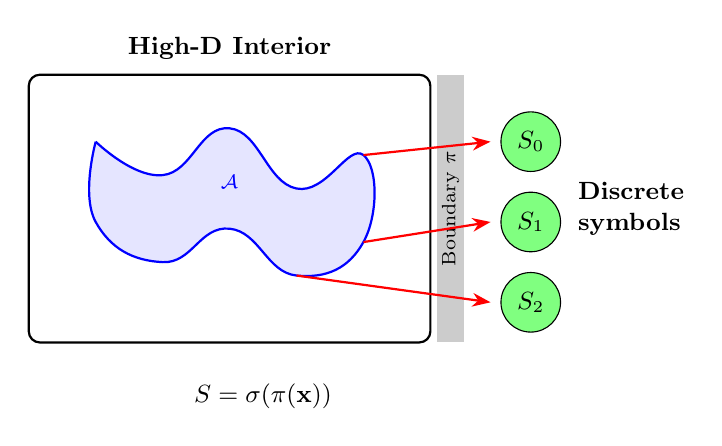
\begin{tikzpicture}[scale=0.85]
    % High-D interior box
    \draw[thick, rounded corners] (-3,-2) rectangle (3,2);
    \node[font=\small\bfseries] at (0,2.4) {High-D Interior};

    % Attractor manifold (wavy shape)
    \draw[thick, blue, fill=blue!10] plot[smooth, tension=0.8] coordinates {(-2,1) (-1,0.5) (0,1.2) (1,0.3) (2,0.8) (2,-0.5) (1,-1) (0,-0.3) (-1,-0.8) (-2,-0.2) (-2,1)};

    % Attractor label - inside the shape
    \node[font=\scriptsize, blue] at (0,0.4) {$\mathcal{A}$};

    % Boundary (right side) - visible bar with label inside
    \fill[gray!40] (3.1,-2) rectangle (3.5,2);
    \node[font=\scriptsize, rotate=90] at (3.3,0) {Boundary $\pi$};

    % Projection arrows - from attractor through boundary
    \draw[-{Stealth}, thick, red] (2,0.8) -- (3.9,1.0);
    \draw[-{Stealth}, thick, red] (2,-0.5) -- (3.9,-0.2);
    \draw[-{Stealth}, thick, red] (1,-1) -- (3.9,-1.4);

    % Discrete outputs - column of symbols
    \node[draw, circle, fill=green!50, minimum size=0.7cm, font=\small] at (4.5,1.0) {$S_0$};
    \node[draw, circle, fill=green!50, minimum size=0.7cm, font=\small] at (4.5,-0.2) {$S_1$};
    \node[draw, circle, fill=green!50, minimum size=0.7cm, font=\small] at (4.5,-1.4) {$S_2$};

    % Output label - to the right
    \node[font=\small, align=left] at (6,0) {\textbf{Discrete}\\\textbf{symbols}};

    % Equation below
    \node[font=\small] at (0.5,-2.8) {$S = \sigma(\pi(\mathbf{x}))$};
\end{tikzpicture}
\caption{Continuous high-dimensional dynamics become discrete symbols at boundaries. The attractor manifold $\mathcal{A}$ projects through boundary $\pi$ onto distinguishable outputs.}
\label{fig:projection}
\end{figure}

\subsection{Mathematical Basis}

The emergence of discrete symbols from continuous dynamics via projection is a consequence of geometry. When a high-dimensional set projects onto a low-dimensional space, the pushforward density is generically non-uniform:

\textbf{Observation (Projection induces structure).} Let $\mathcal{A} \subset \mathbb{R}^n$ be a set traced by entrained dynamics (not necessarily a smooth manifold), and let $\pi: \mathbb{R}^n \to \mathbb{R}^m$ be a linear projection with $m < \dim(\mathcal{A})$. Then for typical $\pi$:
\begin{enumerate}
    \item[(i)] The projected density is non-uniform (clusters and gaps arise from curvature and self-overlap)
    \item[(ii)] Multiple interior states can map to the same boundary value (folds/aliasing)
    \item[(iii)] Sharp density gradients appear where attractor geometry changes orientation relative to the projection
\end{enumerate}

These features---clusters, folds, boundaries---provide the raw material for discretization. A threshold mechanism $\sigma$ converts the clustered projection into discrete symbols.

\textbf{Capacity scaling (heuristic).} The number of distinguishable symbols grows with the dimensionality mismatch. Numerical simulation of coupled oscillator networks suggests rapid growth as the ratio $d/m$ increases, consistent with concentration-of-measure intuitions: high-dimensional distributions concentrate near shells, and projections sample these shells at many distinct angles. The key point is qualitative: high-dimensional attractors ($d \gg 1$) projected onto low-dimensional readouts ($m \sim 1$) produce many distinguishable symbols.

%==============================================================================
\section{The Transition to Life}
%==============================================================================

\subsection{Stage 1: External Organization}

Initially, prebiotic chemistry tracks an \textit{external} attractor---the solar/tidal cycle. The proto-codes that emerge are:
\begin{itemize}
    \item Determined by external forcing
    \item Reproducible under same forcing
    \item History-dependent (initial conditions select position on attractor)
\end{itemize}

The chemistry exhibits information-like behavior, but it is organized \textit{by} the environment, not \textit{by itself}.

\subsection{Stage 2: Compartmentalization}

Lipid bilayers form spontaneously under prebiotic conditions \citep{deamer1985boundary}. Encapsulation produces:
\begin{itemize}
    \item \textbf{Concentration}: Interior chemistry is more concentrated than bulk
    \item \textbf{Defined boundary}: The membrane becomes a specific readout interface
    \item \textbf{Partial decoupling}: Interior dynamics can develop independently of bulk
\end{itemize}

The compartment creates conditions for a qualitative transition.

\subsection{Stage 3: Endogenous Attractor}

The key transition: inside the compartment, some chemistry becomes \textbf{autocatalytic}---self-amplifying reaction networks that can sustain themselves \citep{kauffman1986autocatalytic, hordijk2004detecting}. Such networks, once established, can generate their own dynamics independent of external forcing \citep{england2013statistical}.

Now the interior dynamics can generate their own attractor, independent of external forcing.

\begin{quote}
\textbf{The transition to life}: Swap the external attractor (sun-tracking) for an endogenously generated attractor (self-organization). The ``code'' is now self-maintained.
\end{quote}

\begin{figure}[h]
\centering
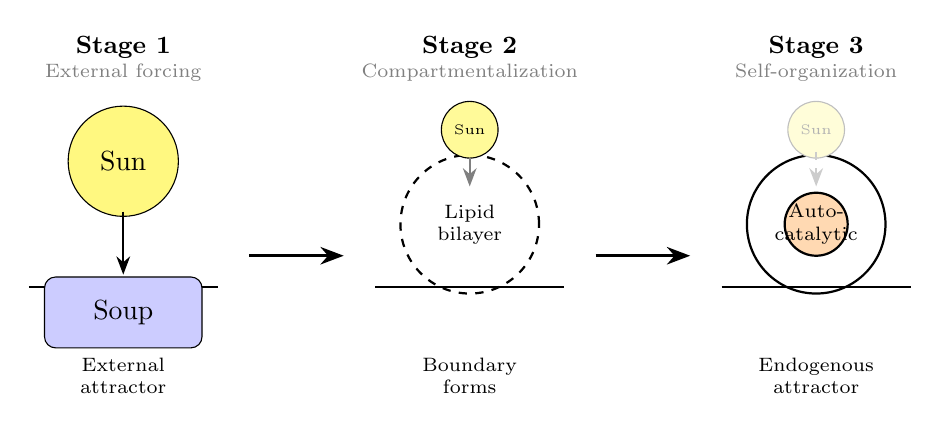
\begin{tikzpicture}[scale=0.8]
    % Stage 1: External forcing dominates
    \node[font=\small\bfseries] at (-4,3.8) {Stage 1};
    \node[font=\scriptsize, gray] at (-4,3.4) {External forcing};
    \draw[thick] (-5.5,0) -- (-2.5,0);
    \node[draw, circle, fill=yellow!50, minimum size=1.4cm] at (-4,2) {Sun};
    \draw[-{Stealth}, thick] (-4,1.2) -- (-4,0.2);
    \node[draw, rounded corners, fill=blue!20, minimum width=2cm, minimum height=0.9cm] at (-4,-0.4) {Soup};
    \node[font=\scriptsize, align=center] at (-4,-1.4) {External\\attractor};

    % Arrow between stages
    \draw[-{Stealth}, very thick] (-2,0.5) -- (-0.5,0.5);

    % Stage 2: Compartmentalization
    \node[font=\small\bfseries] at (1.5,3.8) {Stage 2};
    \node[font=\scriptsize, gray] at (1.5,3.4) {Compartmentalization};
    \draw[thick, dashed] (1.5,1) circle (1.1);
    \node[font=\scriptsize, align=center] at (1.5,1) {Lipid\\bilayer};
    \draw[thick] (0,0) -- (3,0);
    \node[draw, circle, fill=yellow!40, minimum size=0.7cm, font=\tiny] at (1.5,2.5) {Sun};
    \draw[-{Stealth}, thick, gray] (1.5,2.05) -- (1.5,1.6);
    \node[font=\scriptsize, align=center] at (1.5,-1.4) {Boundary\\forms};

    % Arrow between stages
    \draw[-{Stealth}, very thick] (3.5,0.5) -- (5,0.5);

    % Stage 3: Endogenous attractor
    \node[font=\small\bfseries] at (7,3.8) {Stage 3};
    \node[font=\scriptsize, gray] at (7,3.4) {Self-organization};
    \draw[thick] (7,1) circle (1.1);
    \draw[thick, fill=orange!30] (7,1) circle (0.5);
    \node[font=\scriptsize, align=center] at (7,1) {Auto-\\catalytic};
    \draw[thick] (5.5,0) -- (8.5,0);
    \node[font=\scriptsize, align=center] at (7,-1.4) {Endogenous\\attractor};

    % Faded/optional sun (not crude cross-out)
    \node[draw, circle, fill=yellow!15, draw=gray!50, minimum size=0.5cm, font=\tiny, text=gray!60] at (7,2.5) {Sun};
    \draw[-{Stealth}, thick, gray!40, dashed] (7,2.15) -- (7,1.6);

\end{tikzpicture}
\caption{The transition to life. Stage 1: Chemistry tracks external attractor (sun). Stage 2: Compartmentalization creates defined boundary. Stage 3: Internal autocatalytic network generates its own attractor; external forcing becomes optional (faded sun).}
\label{fig:transition}
\end{figure}

This framework dissolves several puzzles:
\begin{itemize}
    \item \textbf{Why codes?} Not designed---emerged from projection
    \item \textbf{Why discrete?} Boundary physics, not chemistry
    \item \textbf{Why self-maintaining?} Attractor swap from external to internal
\end{itemize}

%==============================================================================
\section{Experimental Implications}
%==============================================================================

\subsection{Testing the Framework}

The framework makes specific predictions testable in laboratory settings:

\begin{enumerate}
    \item \textbf{Diversity requirement}: More chemical species $\to$ higher-D attractor $\to$ more distinguishable boundary states. This can be tested by varying mixture complexity.

    \item \textbf{Forcing requirement}: Common forcing is necessary for attractor formation. Without external rhythm, the chemistry equilibrates and loses history-dependence.

    \item \textbf{Boundary discretization}: Different boundary mechanisms (membrane, surface, phase interface) should produce different symbol alphabets from the same interior dynamics.

    \item \textbf{Reproducibility}: Same initial conditions + same forcing $\to$ same boundary state. This is the operational definition of ``code.''
\end{enumerate}

\subsection{Experimental Design}

A minimal test system would include:

\textbf{Substrate}: 20--30 prebiotically plausible species (amino acids, sugars, nucleobases, metal ions, phosphate, fatty acids) in aqueous buffer.

\textbf{Forcing}: UV cycling (simulating day/night) + temperature cycling (20--60$^\circ$C) over periods of hours to days.

\textbf{Boundary}: Lipid vesicles or mineral surface (montmorillonite clay).

\textbf{Readout}: pH indicator dyes or precipitation assays providing discrete outputs.

\textbf{Protocol}:
\begin{enumerate}
    \item Define 32--64 input conditions (forcing phase, initial pH, metal ratios)
    \item Run system for 10--100 forcing cycles
    \item Record boundary state at end of each cycle
    \item Cluster outputs to discover emergent symbols
    \item Measure reproducibility (same input $\to$ same output)
\end{enumerate}

The prediction is that $\geq 32$ distinguishable boundary states emerge without being designed, with reproducibility $> 70\%$.

%==============================================================================
\section{Discussion}
%==============================================================================

\subsection{Prior Experimental Work}

Several experimental traditions have explored related phenomena without the specific framing of boundary-projected code emergence:

\textbf{Oscillating chemical reactions.} Belousov-Zhabotinsky (BZ) systems and coupled oscillator networks exhibit discrete phase states and synchronization \cite{epstein2006introduction}. Showalter and colleagues demonstrated pattern formation and rudimentary computation in BZ droplet arrays. However, this work treats phase states as \textit{computational} rather than as emergent \textit{codes}---no encoding tables are populated, and the question ``how many distinguishable symbols?'' is not asked.

\textbf{Protocell experiments.} Szostak's laboratory demonstrated that lipid vesicles can grow, divide, and selectively concentrate reactants \cite{szostak2001synthesizing}. Deamer showed boundary-mediated chemistry in prebiotic conditions \cite{deamer1985boundary}. These experiments establish that compartmentalization affects chemical dynamics, but focus on \textit{replication} and \textit{metabolism} rather than \textit{information encoding}. No input$\to$output mappings are measured.

\textbf{Autocatalytic networks.} Kauffman's theoretical work on autocatalytic sets \cite{kauffman1993origins}, formalized by Hordijk and Steel \cite{hordijk2004detecting}, shows that self-sustaining reaction networks emerge spontaneously above a complexity threshold. Experimental validation exists for simple RAF (reflexively autocatalytic and food-generated) sets. This addresses ``how does metabolism bootstrap?'' but not ``how do discrete codes emerge from continuous chemistry?''

\textbf{Assembly theory.} Cronin and colleagues developed assembly theory to quantify molecular complexity and demonstrated that complex molecules can form through iterated assembly \cite{cronin2017chemobrionics}. This addresses molecular \textit{complexity} but not informational \textit{discretization}.

\textbf{Our distinction.} We propose a specific \textit{architecture}---high-D substrate, periodic forcing, boundary projection, bistable readout---and a specific \textit{measurement}---encoding/decoding tables populated empirically. The claim is that discrete codes emerge from this architecture as a matter of physics, not that complex chemistry exists (which is well established).

\subsection{Relation to Existing Theories}

Our framework complements rather than contradicts existing origin-of-life theories:

\begin{itemize}
    \item \textbf{RNA World}: RNA could be one of many molecular species tracking external forcing; its eventual dominance reflects its autocatalytic capabilities (Stage 3 transition), not a privileged role in code generation

    \item \textbf{Metabolism-first}: Autocatalytic metabolic cycles are exactly the ``endogenous attractors'' of Stage 3; our framework explains why discrete codes accompany them

    \item \textbf{Lipid World}: Compartmentalization is Stage 2---necessary for the transition but not sufficient; the attractor swap is the key step
\end{itemize}

\subsection{Information Without Observers}

A subtle point: in our framework, ``information'' exists without observers. The boundary states are discrete whether or not anyone reads them. This objective information---distinguishable, reproducible states---is what evolution later learns to use.

This resolves debates about whether information is ``real'' or merely observer-dependent. Emergent digitality is a physical phenomenon: high-D dynamics projected through bistable boundaries produce discrete states as a matter of physics, not interpretation.

\subsection{Implications for Astrobiology}

If codes emerge generically from diverse chemistry + forcing + boundaries, then:
\begin{itemize}
    \item Life-like information processing may be common wherever these conditions obtain
    \item The specific chemistry matters less than the architecture (high-D, forced, bounded)
    \item Detection of extraterrestrial ``life'' might focus on boundary signatures rather than specific molecules
\end{itemize}

%==============================================================================
\section{Conclusion}
%==============================================================================

We have argued that the origin of biological codes is not a problem of engineering but of recognition. Discrete, symbolic information emerges inevitably when:

\begin{enumerate}
    \item High-dimensional chemistry tracks common external forcing (creating attractor manifolds)
    \item Boundaries project this high-D dynamics onto low-D observables (dimensional reduction)
    \item Bistable physical mechanisms discretize the projected outputs (threshold physics)
\end{enumerate}

The transition to life occurs when compartmentalization allows chemistry to swap external attractors for endogenous ones---self-organization replacing sun-organization.

This framework has several virtues:
\begin{itemize}
    \item \textbf{Genericity}: No special chemistry required; any diverse mixture works
    \item \textbf{Inevitability}: Codes emerge from physics, not design
    \item \textbf{Testability}: Specific predictions about diversity, forcing, and boundary effects
    \item \textbf{Parsimony}: Explains discreteness without invoking ``digital chemistry''
\end{itemize}

The genetic code was not invented. It was discovered---at the interface between complex chemistry and simple readouts, where high-dimensional continuous dynamics inevitably project into discrete symbols.

\begin{thebibliography}{99}

\bibitem[Chyba and Sagan(1992)]{chyba1992endogenous}
Chyba, C. and Sagan, C. (1992).
\newblock Endogenous production, exogenous delivery and impact-shock synthesis of organic molecules: an inventory for the origins of life.
\newblock \textit{Nature}, 355(6356):125--132.

\bibitem[Deamer and Oro(1980)]{deamer1985boundary}
Deamer, D.W. and Oro, J. (1980).
\newblock Role of lipids in prebiotic structures.
\newblock \textit{BioSystems}, 12(3-4):167--175.

\bibitem[Eigen(1971)]{eigen1971selforganization}
Eigen, M. (1971).
\newblock Selforganization of matter and the evolution of biological macromolecules.
\newblock \textit{Naturwissenschaften}, 58(10):465--523.

\bibitem[England(2013)]{england2013statistical}
England, J.L. (2013).
\newblock Statistical physics of self-replication.
\newblock \textit{Journal of Chemical Physics}, 139(12):121923.

\bibitem[Epstein and Showalter(1996)]{epstein2006introduction}
Epstein, I.R. and Showalter, K. (1996).
\newblock Nonlinear chemical dynamics: oscillations, patterns, and chaos.
\newblock \textit{Journal of Physical Chemistry}, 100(31):13132--13147.

\bibitem[Hordijk and Steel(2004)]{hordijk2004detecting}
Hordijk, W. and Steel, M. (2004).
\newblock Detecting autocatalytic, self-sustaining sets in chemical reaction systems.
\newblock \textit{Journal of Theoretical Biology}, 227(4):451--461.

\bibitem[Kauffman(1986)]{kauffman1986autocatalytic}
Kauffman, S.A. (1986).
\newblock Autocatalytic sets of proteins.
\newblock \textit{Journal of Theoretical Biology}, 119(1):1--24.

\bibitem[Kauffman(1993)]{kauffman1993origins}
Kauffman, S.A. (1993).
\newblock \textit{The Origins of Order: Self-organization and Selection in Evolution}.
\newblock Oxford University Press.

\bibitem[Miller(1953)]{miller1953production}
Miller, S.L. (1953).
\newblock A production of amino acids under possible primitive earth conditions.
\newblock \textit{Science}, 117(3046):528--529.

\bibitem[Pross(2012)]{pross2012toward}
Pross, A. (2012).
\newblock \textit{What is Life? How Chemistry Becomes Biology}.
\newblock Oxford University Press.

\bibitem[Ruiz-Mirazo et al.(2014)]{ruizmirazo2014prebiotic}
Ruiz-Mirazo, K., Briones, C., and de la Escosura, A. (2014).
\newblock Prebiotic systems chemistry: new perspectives for the origins of life.
\newblock \textit{Chemical Reviews}, 114(1):285--366.

\bibitem[Schr{\"o}dinger(1944)]{schrodinger1944life}
Schr{\"o}dinger, E. (1944).
\newblock \textit{What is Life?}
\newblock Cambridge University Press.

\bibitem[Szostak et al.(2001)]{szostak2001synthesizing}
Szostak, J.W., Bartel, D.P., and Luisi, P.L. (2001).
\newblock Synthesizing life.
\newblock \textit{Nature}, 409(6818):387--390.

\bibitem[Cronin et al.(2017)]{cronin2017chemobrionics}
Cronin, L., et al. (2017).
\newblock Quantifying the origins of life on a planetary scale.
\newblock \textit{Proceedings of the National Academy of Sciences}, 114(49):13202--13207.

\bibitem[Walker and Davies(2013)]{walker2013algorithmic}
Walker, S.I. and Davies, P.C.W. (2013).
\newblock The algorithmic origins of life.
\newblock \textit{Journal of the Royal Society Interface}, 10(79):20120869.

\end{thebibliography}

\end{document}
